\documentclass[12pt,hyperref,a4paper,UTF8]{ctexart}
\usepackage{HDUReport}
\usepackage{listings}
\usepackage{xcolor}
\usepackage{graphicx}
\usepackage{setspace}
\usepackage{float}
\setstretch{1.5} % 设置全局行距为1.5倍

\usepackage{enumitem} % 载入enumitem包以便自定义列表环境
\setlist[itemize]{itemsep=0pt, parsep=0pt} % 设置itemize环境的项目间距和段落间距

\setmainfont{Times New Roman} % 英文正文为Times New Roman


\usepackage{tikz}
\usetikzlibrary{shapes.geometric, arrows}

\tikzstyle{startstop} = [rectangle, rounded corners, minimum width=3cm, minimum height=1cm,text centered, draw=black, fill=red!30]
\tikzstyle{process} = [rectangle, minimum width=3cm, minimum height=1cm, text centered, draw=black, fill=blue!30]
\tikzstyle{decision} = [diamond, minimum width=3cm, minimum height=1cm, text centered, draw=black, fill=green!30]
\tikzstyle{arrow} = [thick,->,>=stealth]

%封面页设置
{   
    %标题
    \title{ 
        \vspace{1cm}
        \heiti \Huge \textbf{《单片机原理及应用》作业报告} \par
        \vspace{1cm} 
        \heiti \Large {\underline{实验报告2第一部分:数据迁移}   } 
        \vspace{3cm}
    
    }

    \author{
        \vspace{0.5cm}
        \kaishu\Large 学院\ \dlmu[9cm]{卓越学院} \\ %学院
        \vspace{0.5cm}
        \kaishu\Large 学号\ \dlmu[9cm]{23040447} \\ %班级
        \vspace{0.5cm}
        \kaishu\Large 姓名\ \dlmu[9cm]{陈文轩} \qquad  \\ %学号
        \vspace{0.5cm}
        \kaishu\Large 专业\ \dlmu[9cm]{智能硬件与系统(电子信息工程)} \qquad \\ %姓名 
    }
        
    \date{\today} % 默认为今天的日期,可以注释掉不显示日期
}
%%------------------------document环境开始------------------------%%
\begin{document}

%%-----------------------封面--------------------%%
\cover
\thispagestyle{empty} % 首页不显示页码
%%------------------摘要-------------%%
%\newpage
%\begin{abstract}




%\end{abstract}

%\thispagestyle{empty} % 首页不显示页码

%%--------------------------目录页------------------------%%
% \newpage
% \tableofcontents
% \thispagestyle{empty} % 目录不显示页码

%%------------------------正文页从这里开始-------------------%
\newpage
\setcounter{page}{1} % 让页码从正文开始编号

%%可选择这里也放一个标题
%\begin{center}
%    \title{ \Huge \textbf{{标题}}}
%\end{center}

\section{原题目}

\textbf{将片外数据存储器地址为1000H~1030H的数据块,全部迁移到片内数据存储器30H~60H中,并将原数据块区域全部清零。用C语言编程。}

\section{实验程序}
\begin{lstlisting}[language=C, caption={数据迁移实验程序}]
#include <reg51.h>

#define EXTERNAL_START  0x1000
#define INTERNAL_START  0x30
#define DATA_LENGTH     49  // 从0x1000到0x1030,共49字节

void main() {
    unsigned char i;
    
    // 1. 初始化片外RAM:写入测试数据
    for (i = 0; i < DATA_LENGTH; i++) {
        *((unsigned char xdata *)(EXTERNAL_START + i)) = i+1;// 存入递增的值
    }

    // 2. 从片外RAM读取,写入片内RAM
    for (i = 0; i < DATA_LENGTH; i++) {
        *((unsigned char idata *)(INTERNAL_START + i)) = *((unsigned char xdata *)(EXTERNAL_START + i));
    }

    // 3. 清零片外RAM
    for (i = 0; i < DATA_LENGTH; i++) {
        *((unsigned char xdata *)(EXTERNAL_START + i)) = 0x00;
    }

    while (1);  // 停止程序运行,便于调试观察
}
\end{lstlisting}

\section{实验效果}

\begin{figure}[H] % [H] 表示强制当前位置插入
    \centering
    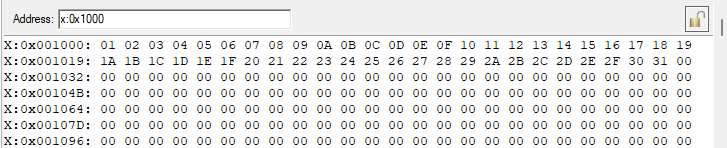
\includegraphics[width=0.8\textwidth]{figures/201.png} % 调整宽度为文本宽度的 80%
    \caption{片外存储器赋值后,内存存储(执行完前13行)} % 图片标题
    \label{fig:example} % 图片标签,用于引用
\end{figure}

\begin{figure}[H] % [H] 表示强制当前位置插入
    \centering
    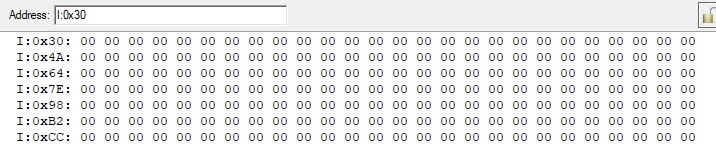
\includegraphics[width=0.8\textwidth]{figures/202.png} % 调整宽度为文本宽度的 80%
    \caption{片内存储器赋值前(执行完前13行)} % 图片标题
    \label{fig:example} % 图片标签,用于引用
\end{figure}

\begin{figure}[H] % [H] 表示强制当前位置插入
    \centering
    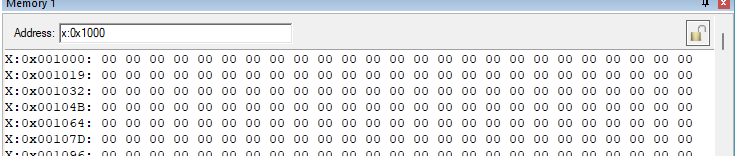
\includegraphics[width=0.8\textwidth]{figures/203.png} % 调整宽度为文本宽度的 80%
    \caption{程序执行完,片外存储器指定区域清零} % 图片标题
    \label{fig:example} % 图片标签,用于引用
\end{figure}

\begin{figure}[H] % [H] 表示强制当前位置插入
    \centering
    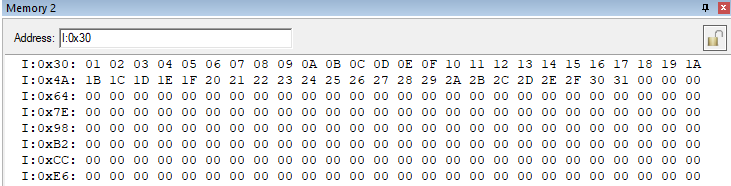
\includegraphics[width=0.8\textwidth]{figures/204.png} % 调整宽度为文本宽度的 80%
    \caption{程序执行完,片内存储器赋值情况} % 图片标题
    \label{fig:example} % 图片标签,用于引用
\end{figure}


\section{流程图}

\begin{figure}[H]
    \centering
    \begin{tikzpicture}[node distance=2cm]

        % Nodes
        \node (start) [startstop] {程序开始};
        \node (init) [process, below of=start] {初始化片外 RAM,写入测试数据};
        \node (transfer) [process, below of=init] {从片外 RAM 读取数据,写入片内 RAM};
        \node (clear) [process, below of=transfer] {清零片外 RAM};
        \node (end) [startstop, below of=clear] {程序结束};

        % Arrows
        \draw [arrow] (start) -- (init);
        \draw [arrow] (init) -- (transfer);
        \draw [arrow] (transfer) -- (clear);
        \draw [arrow] (clear) -- (end);

    \end{tikzpicture}
    \caption{数据迁移程序流程图}
    \label{fig:flowchart}
\end{figure}

\section{实验体会}

实验通过实现片外数据存储器到片内数据存储器的数据迁移,
巩固了对单片机存储器操作的理解。通过编写 C 语言程序,
熟悉了 xdata 和 idata 的使用,初步掌握了片外和片内存储
器的地址映射及数据操作方法。
此外,通过清零片外存储器的操作,理解了数据清理的重要性。
实验还通过观察内存变化验证程序的正确性。总之加深了C51程序的熟练程度。




\end{document}